
\labday{Mercredi, 22 juin 2016}
\label{day:22-06-2016}

\experiment{Compréhension du problème de Transport Optimal}


On dispose de deux distributions de probabilité $\mathcal{P}_S$ et $\mathcal{P}_T$.
On désire projeter la distribution $\mathcal{P}_S$ sur $\mathcal{P}_T$.
Ces distributions sont équipées d'un histogramme (vecteur qui somme à 1) $\mathbf{w}$ et $\mathbf{z}$.
Dans la pratique on dispose de données tirées de ces distributions et pas les 
distributions elles même. 
On a $\mathcal{X}_S$ contenant $n_S$ points tirées de $\mathcal{P}_S$.
Ainsi que $\mathcal{Y}_T$ contenant $n_T$ points tirées de $\mathcal{P}_T$.

Exemple : $\forall i, w_i = (1/n_S)$ et $\forall j, z_j = (1/n_T)$\\
ou encore : $\forall i, w_i = \sum_k e^{-\gamma ||x_i-x_k||^2}$ et $\forall j, z_j = \sum_k e^{-\gamma ||y_j-y_k||^2}$

Le problème de transport optimal consiste à envoyer la distribution $\mathcal{P}_S$ 
sur $\mathcal{P}_T$ à moindre coût.

Avec les mains:\\
On a deux patatoïdes $\mathcal{P}_S$ et $\mathcal{P}_T$. 
On découpe ces patatoïdes en morceau : les points $x_i$ et $y_j$ auxquels on affecte une \emph{masse}
représentée par $\mathbf w$ et $\mathbf z$ tel que la masse de $x_i$ est $w_i$ et la masse de $y_j$ est $z_j$.
On cherche à transférer la masse de $\mathcal{P}_S$ dans $\mathcal{P}_T$ à moindre coût.

\begin{figure}[htbp]
  \centering
  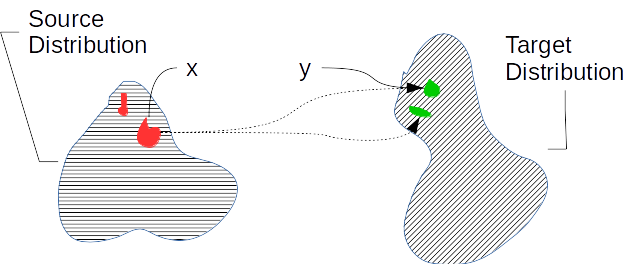
\includegraphics[width=0.95\textwidth]{fig/22-06-2016/ot.png}
  \caption{Illustration d'un problème de transport.}
  \label{fig:label}
\end{figure}

On a besoin d'une matrice de coût $C \in \mathbb{R}^{n_S\times n_T}$ dont 
l'élément $c_{ij}$ indique le coût d'envoyer $x_i$ sur $y_j$ 
(= le coût d'envoyer $w_i$ sur $z_j$)

On cherche à résoudre :

\begin{align}
\min_T \left<T,C\right> = \min_{T} \sum_{ij} t_{ij}*c_{ij}\\
\text{avec}\quad
\forall j, \sum_i t_{ij} = z_j 
\label{mass_in}\\
\forall i, \sum_j t_{ij} = w_i
\label{mass_out}\\
\sum_i w_i = 1
\label{mass_in_tot}\\
\sum_j z_j = 1  
\label{mass_out_tot}
\end{align}

l'équation \eqref{mass_in} signifie que la somme de la masse des éléments $x_i$ de $\mathcal{X}_S$
envoyés sur $y_j$ vaut $z_j$, ie $y_j$ ne reçoit pas plus que sa capacité.

l'équation \eqref{mass_out} signifie que la somme de la masse de $x_i$ envoyé dans les 
éléments $y_j$ de $\mathcal{Y}_T$ vaut $w_i$, ie $x_i$ ne donne pas plus qu'il ne possède.



\subexperiment{Cas 2 points 2D}

On traite le cas simple de 2 points $A\ (x_A, y_A)$ et $B\ (x_B, y_B)$ 
que l'on veux projeter sur $A^\prime\ (x_{A^\prime}, y_{A^\prime})$ et $B^\prime\ (x_{B^\prime}, y_{B^\prime})$ 

On a une matrice de coût :
$$
C = 
\begin{pmatrix}
   c_{AA^\prime} & c_{AB^\prime} \\
   c_{BA^\prime} & c_{BB^\prime} 
\end{pmatrix}
$$

on cherche : 
$$
T = 
\begin{pmatrix}
   t_{AA^\prime} & t_{AB^\prime} \\
   t_{BA^\prime} & t_{BB^\prime} 
\end{pmatrix}
$$
\begin{equation}
\min_T \left<T,C\right> = \min_{T} 
t_{AA^\prime}*c_{AA^\prime} + 
t_{AB^\prime}*c_{AB^\prime} + 
t_{BA^\prime}*c_{BA^\prime} + 
t_{BB^\prime}*c_{BB^\prime}
\end{equation}

\begin{equation}
\left \{
\begin{array}{r c l}
  t_{AA^\prime} + t_{AB^\prime}  & = & 1 \\
  t_{BA^\prime} + t_{BB^\prime}  & = & 1 \\
  t_{AA^\prime} + t_{BA^\prime}  & = & 1 \\
  t_{AB^\prime} + t_{BB^\prime}  & = & 1 \\
\end{array}
\right .
\text{d'où}
\left \{
\begin{array}{r c l}
  t_{AA^\prime}  & = & 1 - t_{AB^\prime}\\
  t_{BB^\prime}  & = & 1 - t_{BA^\prime}\\
  t_{AA^\prime}  & = & 1 - t_{BA^\prime}\\
  t_{AB^\prime}  & = & 1 - t_{BB^\prime}\\
\end{array}
\right .
\text{donc}
\left \{
\begin{array}{r c l}
  t_{AA^\prime}  & = & t_{BB^\prime}\\
  t_{AB^\prime}  & = & t_{BA^\prime}\\
  t_{AA^\prime}  & = & 1 - t_{BA^\prime}\\
\end{array}
\right .
\end{equation}

on définit : $\rho = t_{AA^\prime} = t_{BB^\prime}$ on a $1-\rho = t_{AB^\prime} = t_{BA^\prime}$ et $0\leq \rho\leq 1$

ce qui donne :
$$
T = 
\begin{pmatrix}
   \rho & 1-\rho \\
   1- \rho & \rho
\end{pmatrix}
$$
et le problème devient
\begin{equation}
\min_\rho \rho c_{AA^\prime} + (1- \rho) c_{AB^\prime} + (1-\rho) c_{BA^\prime} + \rho c_{BB^\prime}
\end{equation}
\begin{equation}
\min_\rho \rho (c_{AA^\prime} + c_{BB^\prime} - c_{AB^\prime} - c_{BA^\prime}) + 2
\end{equation}

au final :

\begin{equation}
\rho = \left \{
\begin{array}{r c l}
	1\ \text{si}\ c_{AA^\prime} + c_{BB^\prime} \leq c_{AB^\prime} + c_{BA^\prime} \\
	0\ \text{si}\ c_{AA^\prime} + c_{BB^\prime} \geq c_{AB^\prime} + c_{BA^\prime} \\
\end{array}
\right .
\end{equation}


\subexperiment{Résolution approchée de Cuturi et Courty}

Ici nous allons traité l'algo de \cite{Cuturi2013} utilisé dans \cite{Courty2014},
\cite{Courty2015} utilisant 
l'algorithme de Sinkhorn-Knopp dont la convergence est prouvé dans \cite{Sinkhorn1967} et 
plutôt bien expliqué dans la première partie de \cite{Knight2008} 
(bon après coup il est pas compliqué en fait).


L'approche de Cuturi consiste à ajouter une contrainte à la solution.

\begin{equation}
KL(T||\mathbf{wz}^T ) \leq \gamma
\end{equation}
Où
\begin{equation}
KL(P||Q) = \sum_{ij} p_{ij} \log(\frac{p_{ij}}{q_{ij}} )
\end{equation}
est la divergence de Kullback-Leibler

On introduit alors 3 multiplicateurs de Lagrange : $\lambda, \boldsymbol\alpha, \boldsymbol\beta$.
(Relire les cours sur les SVM)

\begin{equation}
\mathcal{L}(T, \lambda, \boldsymbol\alpha, \boldsymbol\beta) = 
\sum_{ij} t_{ij} c_{ij} + \frac{1}{\lambda} t_{ij} (\log(t_{ij})-\log(w_iz_j))
+ \sum_i \alpha_i (t_{ij}-w_i) + \sum_j \beta_j (t_{ij}-z_j)
\end{equation}
\begin{align}
\forall (i,j),&\quad \frac{\partial \mathcal{L}}{\partial t_{ij}} = 0 \\
\forall (i,j),&\quad \frac{1}{\lambda}\log(t_{ij})+\frac{1-\log(w_iz_j)}{\lambda} + c_{ij} + \alpha_i + \beta_j = 0 \\
\forall (i,j),&\quad -\log(t_{ij}) = 1-\log(w_iz_j) + \lambda c_{ij} + \lambda \alpha_i + \lambda \beta_j \\
\forall (i,j),&\quad t_{ij} = e^{-1+\log(w_iz_j) -\lambda(c_{ij} + \alpha_i + \beta_j )} \\
\forall (i,j),&\quad t_{ij} = w_i e^{-\frac{1}{2}-\lambda\alpha_i} e^{ -\lambda c_{ij}} z_j e^{-\frac{1}{2}-\lambda \beta_j} \\
\end{align}
de plus
\begin{equation}
\left \{
\begin{array}{r c l}
\forall i \quad \frac{\partial \mathcal{L}}{\partial \alpha_i} = 0 \\
\forall j \quad \frac{\partial \mathcal{L}}{\partial \beta_j} = 0 \\
\quad \frac{\partial \mathcal{L}}{\partial \lambda} = 0 \\
\end{array}
\right .
\left \{
\begin{array}{l}
\forall i \quad t_{ij}-w_i = 0 \\
\forall j \quad t_{ij}-z_j = 0 \\
\sum_{ij} \frac{-1}{\lambda^2} t_{ij} (\log(t_{ij})-\log(w_iz_j)) = 0 \\
\end{array}
\right .
\left \{
\begin{array}{l}
\forall i \quad t_{ij} = w_i \\
\forall j \quad t_{ij} = z_j \\
\sum_{ij} (\log(t_{ij})-\log(w_iz_j)) = 0\\
\end{array}
\right .
\end{equation}

Ainsi $T_\lambda$ est, selon le théorème de Sinkhorn et Knopp, 
l'unique matrice dont les lignes sommes à $\mathbf{w}$ 
et les colonnes à $\mathbf{z}$ ayant la forme:

\begin{equation}
  \exists \mathbf{u},\mathbf{v} > \mathbf{0}_d : T^\lambda = diag(\mathbf{u}) e^{-\lambda C} diag(\mathbf{v})
\end{equation}

$\mathbf w$, $\mathbf z$, $\boldsymbol\alpha$ et $\boldsymbol\beta$ ont été absorbé par $\mathbf{u}$ et $\mathbf{v}$. C'est magique.


Maintenant, tous les éléments de $T$ sont calculables sous condition d'avoir $e^{-\lambda C},\mathbf w,\mathbf z$.
$diag(\mathbf{u})$ et $diag(\mathbf{v})$ sont données par l'algo de Sinkhorn-Knopp
(à partir de $\mathbf w$ et $\mathbf z$)
qui consiste à re-normaliser alternativement les lignes et les colonnes jusqu'à 
convergence (à $\epsilon$ près).


%----------------------------------------------------------------------------------------
